\documentclass[hyperref={pdfpagelabels=false},t,10pt]{beamer}
\usepackage[utf8]{inputenc}
\usepackage[english]{babel}
\usepackage[T1]{fontenc}
\usepackage[default,scale=.95]{opensans}


\usetheme[cd2018]{tud}
\setbeamercolor{normal text}{fg=black}
\colorlet{alert}{cdblue}
\setbeamercolor{alerted text}{fg=cdblue}
\setbeamerfont{frametitle}{size=\Large,family=\sffamily,series=\sbseries}


\DeclareRobustCommand\sbseries{\fontseries{sb}\selectfont}
\DeclareTextFontCommand{\textsb}{\sbseries}


\title{TITLE}
\author[© author]{Maik Thanh Nguyen}
\institute{Technische Universit\"at Dresden}
\datecity{CONFERENCE}
\date{DATE}


\begin{document}

%%%% Uncomment the following line to set background image to main slide
%%%% (parameter sets transparency)
%\setbeamertemplate{tud background}[image/shaded]{background.jpg}{0.5}
\addtocounter{framenumber}{-1}
\maketitle

\begin{frame}
  \frametitle{Content}

  \begin{itemize}
  \item Modal logic and semantics
    \begin{itemize}
        \item Kripke frames
        \item Topological space
        \item Neighbourhood frames
     \end{itemize}
  \item Multimodal logic and product of frames/spaces and logics
    \begin{itemize}
      \item Notation, Fusion of logics
      \item Horizontal and Vertical topology/functions
      \item Product of logics and the logic T
    \end{itemize}
  \item Main result and ideas
  \end{itemize}
\end{frame}

\begin{frame}
  \frametitle{Modal logic and Kripke frames and models}
  \begin{itemize}
    \item Modal logic extends classical propositional logic. Formally:
    $$\phi ::= p \mid \bot \mid \neg \phi \mid \phi \lor \phi \mid \Box \phi$$
    where $\Box$ is a modal operator and Prop is a set of variable with $p \in$ Prop.
    %Other connectives are expressed through $\neg$ and $\lor$ and dual modal operator $\lozenge$ as $\lozenge \phi = \neg \Box \neg \phi$. 
     \pause

    \item A frame $F = (W,R)$ is a pair where 
    \begin{itemize}
      \item $W$ is a non-empty set of worlds
      \item $R \subseteq W \times W$ is a binary relation  
    \end{itemize}

    \item A model is a pair $M = (F,R)$ ($M$ is based on $F$) where
      \begin{itemize}
        \item $F$ is a frame
        \item $V$ is a valuation and is of the form $V : Prop \rightarrow 2^W$
      \end{itemize}
  \end{itemize}
\end{frame}

\begin{frame}
  \frametitle{Kripke semantics}
  \begin{itemize}
    \item Let $M = (F,V)$ be a model and $w \in W$ a state in $M$. A formula being true at $w$ is inductively defined as: 
  \end{itemize}

  \begin{align*}
    M, w &\Vdash p &&\text{ iff } w \in V(p) \\
    M, w &\Vdash \bot  &&\text{ never } \\
    M, w &\Vdash \neg \phi &&\text{ iff not } M, w \Vdash \phi \\ 
    M, w &\Vdash \phi \lor \psi &&\text{ iff } M,w \Vdash \phi \lor M,w \Vdash \psi \\
    M, w &\Vdash \Box \phi &&\text{ iff } \forall v \in W : wRv \rightarrow M, v \Vdash \phi \\
    M, w &\Vdash \lozenge \phi &&\text{ iff } \exists v \in W : wRv \land M,v \Vdash \phi
\end{align*}
  
\end{frame}

\begin{frame}
  \frametitle{Example}
  \begin{itemize}
    \item Let $\phi = \Box p$ and $M = (W,R,V)$ with $W = \{w_1,w_2,w_3,w_4,w_5\}$, $V(p) = \{w_3,w_4,w_5\}$ and $R = $
  \end{itemize}
  \centering
  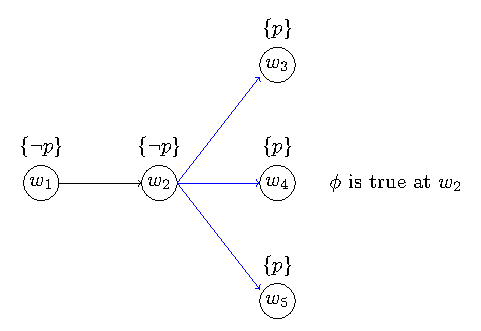
\includegraphics[width=0.55\textwidth]{Example1.pdf}
  \pause
  \begin{itemize}
    \item Kripke semantics has many applications for example epistemic logic, temporal logic,...
  \end{itemize}
\end{frame}

\begin{frame}
  \frametitle{Motivation topological space}
  \begin{itemize}
    \item We want to reason not just about "what is true" but "where is true" \pause
    \item Topological space deals with open sets, it can describes which points are "nearby"
    \item applications: spatial reasoning %for example reasoning about neighboring regions or reachability (AI, robotics)
    \end{itemize}
    \end{frame}


    \begin{frame}
      \frametitle{Topological space}
      \begin{itemize}
            \item A topological space is a pair $(X, \tau)$, where $\tau$ (called topology) is a collection of subsets of $X$ (open sets) such that: 
        \begin{itemize}
          \item $\emptyset$ and $X$ are open
          \item the union of arbitrary collection of open sets is open
          \item the intersection of finite collection of open sets is open
        \end{itemize}
          \item A topological model is a structure $M = (X,\tau, \upsilon)$ where $(X, \tau)$ is a topological space and $\upsilon$ a valuation of the form $\upsilon : Prop \rightarrow 2^X$ 
      \end{itemize}
  \end{frame}

\begin{frame}
  \frametitle{Topological semantics}
  Let $M = (X, \tau, \upsilon)$ be a topological model and $x \in X$ a point in $M$. A formula being true at $x$ is inductively defined as:

  \[
\begin{aligned}
    M, x &\vDash p &&\text{iff } x \in v(p) \\
    M, x &\vDash \bot &&\text{never} \\
    M, x &\vDash \neg \phi &&\text{iff } M, x \nvDash \phi \\
    M, x &\vDash \phi \lor \psi &&\text{iff } M, x \vDash \phi \text{ or } M, x \vDash \psi \\
    M, x &\vDash \Box \phi &&\text{iff }\exists U \in \tau \text{ such that } x \in U \text{ and } \forall u \in U,\; M, u \vDash \phi \\
    M, x &\vDash \lozenge \phi &&\text{iff }\forall U \in \tau: \text{if }x \in U \rightarrow \exists u \in U,\; M, u \vDash \phi
\end{aligned}
\]

\end{frame}

\begin{frame}
  
  \frametitle{Example}
  \begin{itemize}
    \item  Let $(X,\tau)$ be a topological space with 
    $X = \{1,2,3\}$, $\tau = \{\emptyset, \{1\}, \{2\}, \{1,2\}, W\}$ and $V(p) = \{1,2\}$. Furthermore, let $\phi = \Box p$.
    \pause
  \end{itemize}
  \centering
  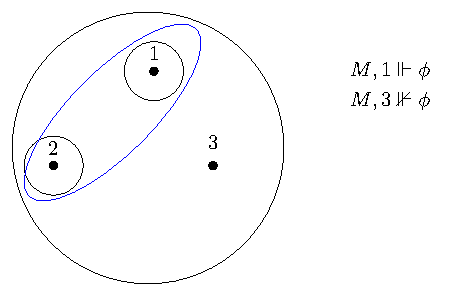
\includegraphics[width=0.55\textwidth]{Example2.pdf}
\end{frame}


\begin{frame}
  \frametitle{Neighbourhood frames}
  \begin{itemize}
    \item generalize Kripke semantics
    \item captures non-normal modal logics
    \item application in Epistemic logic
    \pause
    \item A neighbourhood frame is a pair $(X, \tau)$ where $\tau$ is a function $\tau : X \rightarrow 2^{2^X}$.
    \item A neighbourhood model is a structure $M = (X, \tau, \upsilon)$, where $\upsilon$ is a valuation of the form $\upsilon : Prop \rightarrow 2^X$
  \end{itemize}
\end{frame}

\begin{frame}
  \frametitle{Neighbourhood semantics}
  Let $M = (X,\tau,\upsilon)$ be a neighbourhood model and $x \in X$ a point in $M$. A formula being true at x is inductively defined as:
      \begin{align*}
        M,x &\Vdash p &&\text{iff } x \in V(p)\\
        M,x &\Vdash \bot &&\text{never } \\
        M,x &\Vdash \neg \phi &&\text{iff } M,x \nVdash \phi\\
        M,x &\Vdash \phi \lor \psi &&\text{iff } M,x \vDash \phi \lor M,x \vDash \psi\\
        M,x &\Vdash \Box \phi &&\text{iff } \exists V \in \tau(x) \forall y \in V : M,y \models \phi
    \end{align*}

\end{frame}

\begin{frame}
  \frametitle{Example}
      Assume $\phi = \Box p$. Let $W = \{1,2,3\}$, $V(p) = \{1,2\}$ and 
    \[
            \tau(x) = 
            \begin{cases}
                1 \rightarrow \{\{1\}, \{3\}, W\} \\
                2 \rightarrow \{\{2\}, \{1,2\}, W\} \\
                3 \rightarrow \{\{3\}, \{1,3\}\}
            \end{cases}
    \] 
    \centering
      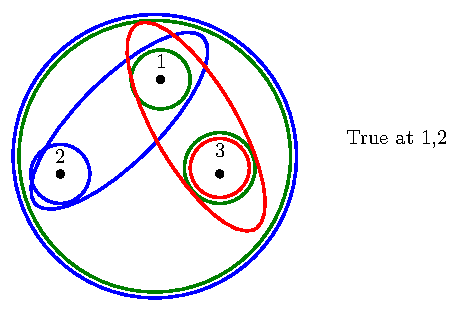
\includegraphics[width=0.55\textwidth]{Example3.pdf}
\end{frame}

\begin{frame}
  \frametitle{Multimodal logic and product of frames}
  \begin{itemize}
    \item Mutlimodal logic allows us to reason about knowledge,time etc. simultaneously 
    \item for example we can combine temporal and epistemic logic to reason about "when does the agent knows something" (product of frames) \pause
    \item horizontal and vertical relation allows us to reason in one dimension% , for example we a fix time point and ask what does the agent knows at that time?
    \item Let $F = (W, R_1)$ and $G = (V, R_2)$. We define the Kripke product on $W \times V$as : 
      $$(w,v)R_1'(w',v') \mbox{ iff } wR_1w' \mbox{ and } v = v' \text{  (horizontal)}$$
      $$(w,v)R_2  '(w',v') \mbox{ iff } w = w' \mbox{ and } vR_2v' \text{(vertical)}$$
    %\item Let $L_1$ and $L_2$ be two modal logics with one modality $\Box$. Then the fusion
    %is defined as: $$L_1 \otimes L_2 = K_2 + L_{1 \Box \rightarrow \Box_1} + L_{2 \Box \rightarrow \Box_2}$$
   % \item we consider the product of frames to evaluate multimodal formulas
  \end{itemize}
\end{frame}

\begin{frame}
  \frametitle{Fusion}
  \begin{itemize}
    \item we can also combine logics with fusion
    \item Let $L_1$ and $L_2$ be modal logics with one modality $\Box$. Then the fusion is defined as:
    $$ L_1 \otimes L_2 = K_2 + L_{1(\Box \rightarrow \Box_1)} L_{2(\Box \rightarrow \Box_2)} $$ 

  \end{itemize}

\end{frame}

\begin{frame}
  \frametitle{Horizontal and Vertical topology}
  \begin{itemize}
    \item in topological space, horizontal and vertical can be also defined 
  \end{itemize}
  Let \( \mathcal{X} = (X, \chi) \) and \( \mathcal{Y} = (Y, \upsilon) \) be topological spaces and \( N \subseteq X \times Y \) \newline

\begin{description}
  \item[Horizontally open:] \(N\) is horizontally open iff 
  \[
    \forall (x, y) \in N\; \exists U \in \chi \text{ such that } x \in U \text{ and } U \times \{y\} \subseteq N.
  \]

  \item[Vertically open:] \(N\) is vertically open iff 
  \[
    \forall (x, y) \in N\; \exists V \in \upsilon \text{ such that } y \in V \text{ and } \{x\} \times V \subseteq N.
  \]

\end{description}

$\tau_1$ (horizontal topology) is the set of all horizontally open sets and $\tau_2$ (vertical topology) the set of all vertically open sets.


\end{frame}

\begin{frame}
  \frametitle{Illustration, standard product}
    \centering
    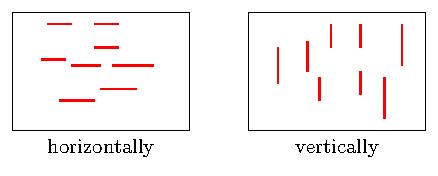
\includegraphics[width=0.55\textwidth]{Example4.pdf}
  \begin{itemize}
    \item we can also reason in both directions at once with the standard topology
    \item we denote the standard toplogy as $\tau$ where 
    $$\tau = \{N \subseteq X \times Y \mid \exists U \in \chi \exists V \in \upsilon: N = U \times V\}$$  
  \end{itemize}

\end{frame}

\begin{frame}
  \frametitle{horizontal, vertical and standard functions}
  Let $\mathcal{X}$ = ($X$, $\tau_1$) and $\mathcal{Y}$ = ($Y$, $\tau_2$) be two n-frames. We define the full product as
    $$\mathcal{X} \times_n^+  \mathcal{Y} = (X \times Y, \tau_1', \tau_2', \tau) \text{ where}$$
    $$ \tau_1'(x,y) = \{ U \subseteq \mbox{X} \times \mbox{Y} \mid \exists V \in \tau_1(x) : V \times  \{ y \} \subseteq U \}$$
    $$ \tau_2'(x,y) = \{ U \subseteq \mbox{X} \times \mbox{Y} \mid \exists V \in \tau_2(y) : \{ x \} \times V \subseteq U \}$$
        $$ \tau(x,y) = \{ U \subseteq \mbox{X} \times \mbox{Y} \mid \exists W \in \tau_1(x) \, \exists V \in \tau_2(y) : W \times V \subseteq U \}$$   
\end{frame}

\begin{frame}
  \frametitle{Product of logics and the logic T}
  Let $L_1$ and $L_2$ be two unimodal logic. We define the full n-product of them as:
  $$L_1 \times_n^+ L_2 =  Log(\{\mathcal{X} \times_n^+ \mathcal{Y} \mid \mathcal{X} \Vdash L_1 \text{ and } \mathcal{Y} \Vdash L_2 \})$$ \pause
  \begin{itemize}
    \item this thesis deals with the logic $T$
    \item $T = K + \Box p \rightarrow p$
  \end{itemize}
\end{frame}

\begin{frame}
  \frametitle{Main Research Question}
  \begin{itemize}
    \item Does the following equality holds? 
    $$T \otimes T \otimes T + \Box p \rightarrow \Box_1 p \land \Box_2 p = T \times_n^+ T$$
    where $T \otimes T \otimes T = K_3 + T_{\Box} + T_{(\Box \rightarrow \Box_1)} + T_{(\Box \rightarrow \Box_2)}$ is the logic with three modalities 
    and $\Box p \rightarrow \Box_1 p \land \Box_2 p$ the interaction axiom
    \item main motivation comes from epistemic logic 
    \item We will only sketch completeness w.r.t. to the class of frames
  \end{itemize}
\end{frame}

\begin{frame}
  \frametitle{Sketch of the main ideas}
  

\end{frame}
\end{document}
